\shorthandoff{:!} %règle un problème de compatibilité avec babel
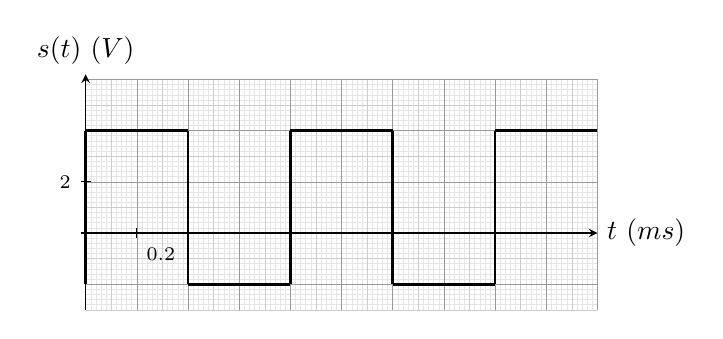
\begin{tikzpicture}[scale=0.65]
	%papier milli
	\draw [very thin, gray!20] (0,-1.5) grid[step=0.1] (10,3);
	\draw [very thin, black!20] (0,-1.5) grid[step=0.5] (10,3);
	\draw [very thin, black!40] (0,-1.5) grid[step=1] (10,3);
	%fin 
	%axes
	\draw[->,>=stealth] (-0.1,0) -- (10,0) node[right] {$t\ (ms)$};
	%stealth définit un style de flèche, "furtif"
	\draw[->,>=stealth] (0,-1.5) -- (0,3.1)node[above] {$s(t)\ (V)$};
	\draw (1,0.1) -- (1,-0.1) node [below right] {{\scriptsize $0.2$}}; %échelle abscisse
	\draw (0.1,1) -- (-0.1,1) node [left] {{\scriptsize $2$}}; %échelle ordonnée
	%fin
	%lLe signal
	\draw [color=black,line width=1pt, smooth] (0,2) -- (2,2);
	\draw [color=black,line width=1pt, smooth] (2,-1) -- (4,-1);
	\draw [color=black,line width=1pt, smooth] (4,2) -- (6,2);
	\draw [color=black,line width=1pt, smooth] (6,-1) -- (8,-1);
	\draw [color=black,line width=1pt, smooth] (0,-1) -- (0,2);
	\draw [color=black,line width=1pt, smooth] (2,-1) -- (2,2);
	\draw [color=black,line width=1pt, smooth] (4,-1) -- (4,2);
	\draw [color=black,line width=1pt, smooth] (6,-1) -- (6,2);
	\draw [color=black,line width=1pt, smooth] (8,-1) -- (8,2);
	\draw [color=black,line width=1pt, smooth] (8,2) -- (10,2);

\end{tikzpicture} 
\shorthandon{:!}